\chapter{計算氫分子的電子結構}\label{ch:first}

氫分子只有兩個原子，卻包含一次電子結構計算中最基本的幾個問題：原子放在哪裡，電子怎樣分佈，怎樣知道計算已經結束，以及所得數字究竟對應哪一種結構。本章從一個準備好的結構檔案出發，完成自洽場計算，並閱讀能量和誤差曲線。完成本章後，便可用相同的方法處理較大的分子或晶體。

本例使用平面波和贗勢方法。對於第一次操作，不必先掌握這些方法的數學推導。先認識介面中的結構、節點和結果，觀察它們之間的關係，再閱讀第\ref{ch:theory}章，通常更容易理解各個引數的作用。

\section{準備氫分子算例}

我們在一個立方形模擬盒中放入兩個氫原子，保持原子位置不變，求解它們在這一位置上的基態電子分佈。這是一項單點能計算。“單點”表示只計算一個幾何構型，並不表示只進行一次數值迭代。電子密度需要反覆更新，直到前後兩次計算足夠接近，這個過程稱為自洽場計算，通常簡寫為 SCF。

本章完成時，專案中應包含一個氫分子結構、一張可以再次執行的工作流，以及一幅能量和誤差曲線。同時儲存專案，以便在後面的結構最佳化教程中繼續使用。第一次操作可使用當前工作區的計算環境；線上版在伺服器會話中執行相同步驟。

\begin{table}[htbp]
\centering
\caption{氫分子教程的計算條件}
\begin{tabularx}{\linewidth}{lX}
\toprule
專案 & 本例設定\\
\midrule
結構型別 & Molecule\\
模擬盒 & 邊長為 $10$ Bohr 的立方盒，即約 $5.29177$ Å\\
氫原子位置 & 分數座標 $(0.5,0.5,0.425)$ 和 $(0.5,0.5,0.575)$\\
初始鍵長 & $1.5$ Bohr，約 $0.793766$ Å\\
交換關聯泛函 & PBE\\
贗勢 & default，內建 PBE-1.3 ONCV 贗勢\\
平面波截斷能 & $20$ Ha\\
自旋分量數 & Nspin = 1\\
溫度 & $0$ K\\
SCF 方法 & davidson\_qe；最大 $100$ 步\\
力 & 選中 Calculate force\\
\bottomrule
\end{tabularx}
\end{table}

教程檔案 \file{examples/h2.cif} 儲存了上述模擬盒和原子位置。使用這個檔案，可以避免手工輸入座標，也能使桌面版和線上版的起始結構保持一致。CIF 的晶格描述在此用於儲存模擬盒；計算時仍需在 \ui{Build Molecule} 節點中選擇 \ui{Molecule}。檔案格式和計算物件的型別是兩件不同的事。

\begin{notebox}{為什麼選擇一個很小的分子}
小體系便於觀察每一步操作，也便於比較引數變化的影響。本例給出盒尺寸和截斷能，便於完成計算並比較結果。換用其他分子時，應重新檢查這兩個引數的收斂性。
\end{notebox}

\section{建立專案並匯入結構}

\subsection{為計算建立一個單獨的專案}

專案把結構、工作流和結果放在一起。一個清楚的專案名稱，有助於在幾天後重新開啟檔案時迅速判斷它的用途。這裡可以使用“氫分子入門”，並把專案儲存為 \file{h2-first.ks}。應用啟動時已有一個空專案；如果當前開啟了其他專案，先儲存原有工作，再關閉該專案，返回新的空專案。

\begin{steps}
\item 如當前已有其他專案，先儲存，再選擇 \ui{主頁 → 關閉}。
\item 在專案瀏覽器中確認已經出現結構、工作流和結果等分類。
\item 保持空專案處於開啟狀態，繼續匯入結構。
\item 匯入完成後選擇 \ui{儲存}，為專案指定名稱和位置。
\end{steps}

桌面版通常透過系統檔案對話方塊選擇本地檔案。線上版的檔案選擇和下載經過瀏覽器完成：先把教程檔案提供給當前會話，再在應用中選擇它。無論在哪一種環境中，匯入後的結構都應出現在專案瀏覽器裡，而不是僅僅停留在瀏覽器的下載列表中。

\subsection{匯入氫分子}

\begin{steps}
\item 在 \ui{主頁} 的結構命令中選擇 \ui{從檔案匯入結構}。
\item 選擇教程提供的 \file{h2.cif}。
\item 在專案瀏覽器中選中匯入的結構，展開同側的 \ui{資訊瀏覽器} 標題欄，檢查元素和原子數量。面板未顯示時，從省略號中的 \ui{開啟面板} 列表按名稱開啟。
\item 開啟結構的三維檢視，旋轉模型，使兩個氫原子都清楚可見。
\end{steps}

此時應當看到兩個氫原子。模擬盒的邊界可能同時顯示，也可能根據當前顯示設定隱藏。球的大小和鍵的畫法隻影響顯示，不會改變原子座標。若結構超出畫面或偏離中心，使用檢視器的適配檢視或縮放功能即可。

\subsection{確認幾何資訊}

在繼續計算之前，先用檢視器的距離測量檢查兩個氫原子的間距。輸入結構的初始鍵長約為 $0.793766$ Å。檢視器顯示的小數位數可能不同，讀到 $0.794$ Å 即與這裡的輸入相符。與之對應的底層座標單位是 Bohr，鍵長為 $1.5$ Bohr。

也可以選擇一個氫原子，檢查座標卡片。圖\ref{fig:h2-structure-inspection}選擇的是第2個位點，其分數座標為 $(0.500,0.500,0.575)$，對應的笛卡爾座標顯示為 $(2.646,2.646,3.043)$ Å。前者表示原子在模擬盒中的相對位置，後者表示以 Å 為單位的實際位置。原子處於盒子中部，四周留有空間。CIF 匯入後的結構文件可以顯示\ui{晶體建模}頁面；後續求解仍按本章要求在結構配置節點選擇\ui{Molecule}。

\begin{figure}[!htb]
\centering
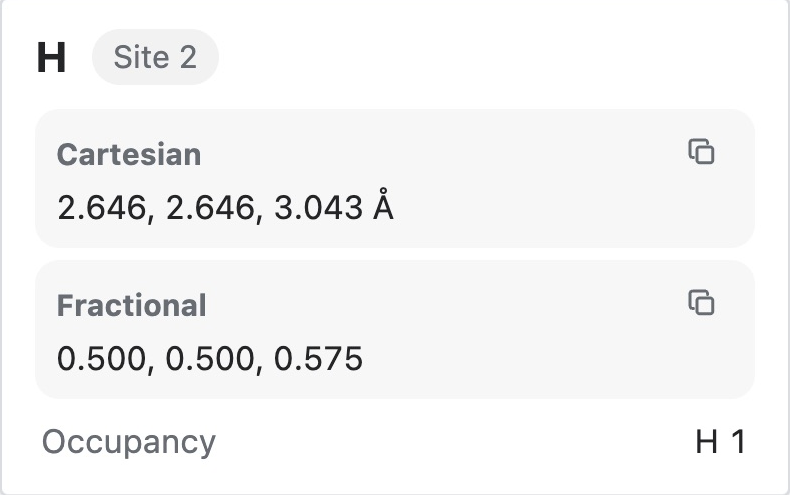
\includegraphics[width=79mm]{publication-assets/crop-f7556efd0d7de78b7cf1.png}
\caption{初始氫分子第2個位點的座標卡區域性，顯示笛卡爾座標、分數座標與佔位。座標卡用於核對所選位點的幾何資訊。}
\label{fig:h2-structure-inspection}
\end{figure}

電子結構計算取決於原子位置。本例核對兩個氫原子、約 $0.794$ Å 的鍵長和約 $5.292$ Å 的立方盒即可。

如果使用自己的 XYZ 檔案建立相同的氫分子，原子間距可以相同，模擬盒卻未必相同。分子檔案沒有晶格時，軟體會根據原子範圍和真空距離構造盒子。要與本章數字作細緻比較，應使用相同的模擬盒，而不僅是相同的鍵長。

\section{建立自洽計算工作流}

\subsection{從 \headinglatin{SCF} 模板開始}

工作流把計算過程分為若干節點。節點之間的連線表示處理順序。本例只需要三項工作：把匯入的結構交給求解器、計算電子結構、顯示收斂過程。使用模板可以先得到這套基本關係，再逐項調整其中的引數。

\begin{steps}
\item 開啟 \ui{工作流} 的匯入選單，選擇 \ui{從模板建立工作流}。
\item 選擇 \ui{SCF} 模板。
\item 開啟新建的工作流文件，檢視畫布上的節點和連線。
\item 確認工作流包含結構配置、SCF 計算和能量曲線三個任務，並按這一順序連線。結構配置節點的標籤可以是\ui{Configuration}或\ui{Build Molecule}，對應同一任務；後兩個節點依次為\ui{SCF}和\ui{Plot}。
\end{steps}

若選擇的是空白工作流，可以自行新增上述三個節點，再依次連線。節點的顯示名稱可以修改，任務型別則應保持正確。例如，把節點標籤改為“計算氫分子”不會改變它是一個 SCF 任務。對於第一次操作，保留模板名稱更容易與本章說明對應。

可以對照圖\ref{fig:h2-workflow}檢查順序：第一個節點接收結構，第二個節點完成電子結構求解，最後一個節點讀取計算歷史並畫出曲線。接下來按這個順序逐項配置。

\begin{figure}[!htb]
\centering
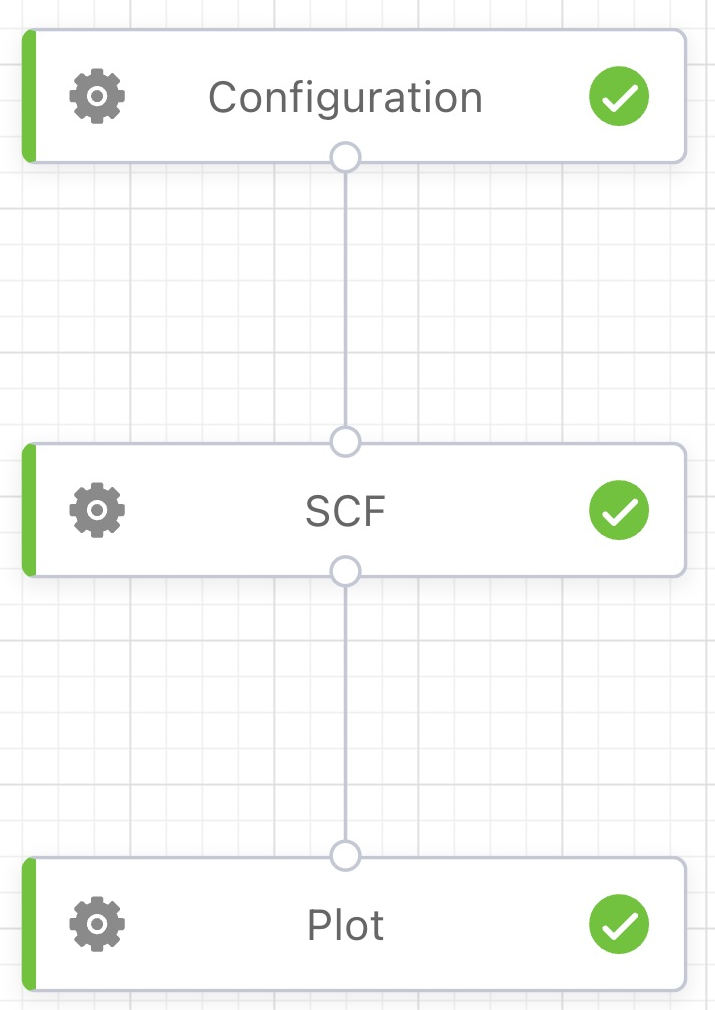
\includegraphics[width=60mm]{publication-assets/crop-273037e846506daab173.png}
\caption{氫分子的SCF工作流。結構配置、電子結構求解和繪製曲線自上而下連線；Configuration對應Build Molecule任務，Plot對應繪製收斂曲線。}
\label{fig:h2-workflow}
\end{figure}

\subsection{配置結構輸入}

在畫布上選擇結構配置節點\ui{Configuration}，再選擇 \ui{工作流 → 配置節點}，也可以使用節點上的齒輪。這項命令會展開原本收起的右側面板，並在 \ui{配置編輯器} 中開啟或重新整理該節點的專用設定；向下滾動到 \ui{選項} 區，便可以看到 Type 等引數。只看到節點 ID、標籤、模組等通用屬性時，請先執行配置節點命令。這個節點既指定結構，也規定求解時採用的物理和數值模型。執行前，按本例設定逐項核對結構與計算引數。

如果面板較窄，引數名稱或下拉框內容可能被截短。點選\ui{配置編輯器}標題欄右上角的省略號，選擇\ui{最大化}，可以暫時把主要工作區讓給這個面板。完成填寫後，再從同一選單選擇\ui{還原}，回到畫布與引數並列的佈局。\ui{通用}、\ui{輸入}、\ui{選項}和\ui{高階選項}各自可以展開或摺疊；填寫本例時，可先摺疊通用與輸入，把空間留給選項。

\begin{steps}
\item 將 \ui{Type} 設為 \ui{Molecule}。
\item 在 \ui{Choose imported structures} 中只選擇本例的氫分子。
\item 將 \ui{Functional} 設為 \ui{PBE}，\ui{Pseudopotential} 設為 \ui{default}。
\item 在 \ui{Ecut (Hartree)} 中輸入 \texttt{20}。
\item 保持 \ui{Smearing} 為 \ui{fermi-dirac}，\ui{Temperature (K)} 為 \texttt{0}，\ui{Nspin} 為 \texttt{1}。
\item 在高階選項中保持額外能帶數為 \texttt{0}。
\end{steps}

選擇 Molecule 後，晶體的自動 k 點設定不再是本例需要調整的內容。本例採用盒內分子模式，無須設定晶體的 k 點網格。

\ui{Ecut (Hartree)} 中的單位尤其值得留意。這裡輸入 $20$ 表示 $20$ Ha，約合 $544$ eV；它並不是 $20$ eV。圖形介面把單位寫在標籤裡，閱讀論文或其他軟體的輸入時，也應先完成單位換算，再比較引數大小。

\begin{figure}[H]
\centering
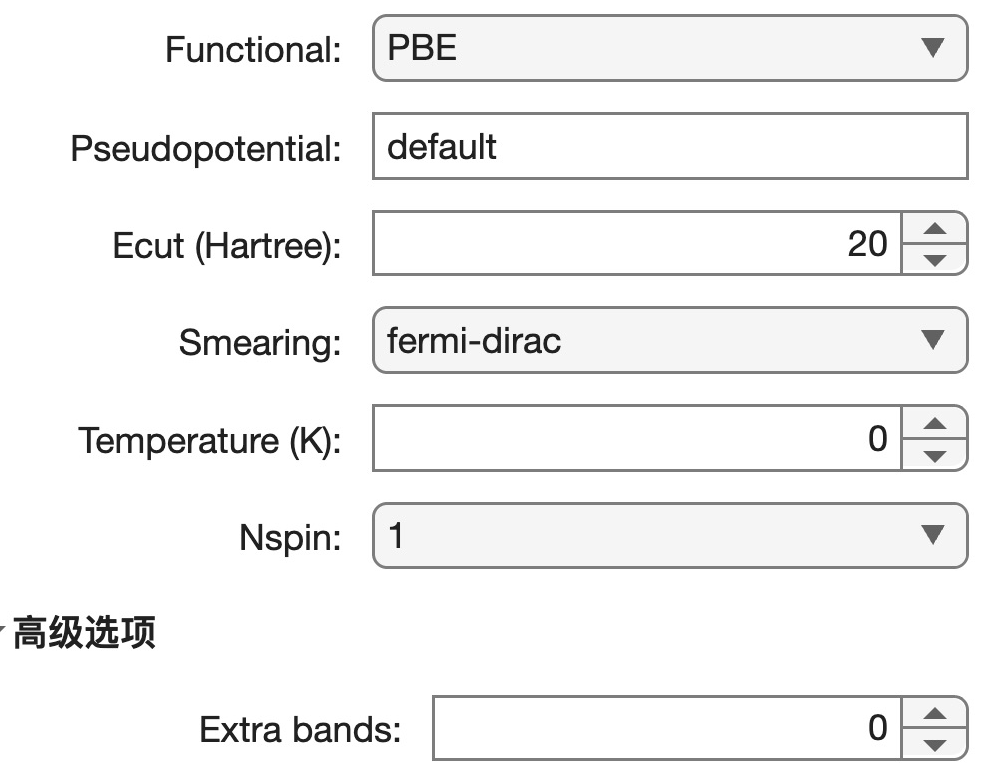
\includegraphics[width=90mm]{publication-assets/crop-1d148adc90da2955994e.png}
\caption{結構配置節點的常規與高階選項。PBE、default贗勢、20 Ha、0 K、Nspin=1和Extra bands=0均可在此核對；Molecule與結構h2的選擇見圖\ref{fig:online-h2-config}。}
\label{fig:h2-build-options}
\end{figure}

\subsection{配置 \headinglatin{SCF} 節點}

選擇 \ui{SCF} 節點，再選擇 \ui{工作流 → 配置節點}，向下滾動到它的 \ui{選項} 區。\ui{DiagMethod} 決定每一步求解電子態時使用的數值方法；\ui{Max SCF steps} 則規定電子密度最多更新多少次。對於本例，使用預設的 \ui{davidson\_qe} 和 $100$ 步即可。

展開\ui{DiagMethod}下拉框時，可以看到多種方法。本例選擇\ui{davidson\_qe}；收起後如果文字顯示不全，可最大化面板核對完整名稱。

\begin{figure}[!htb]
\centering
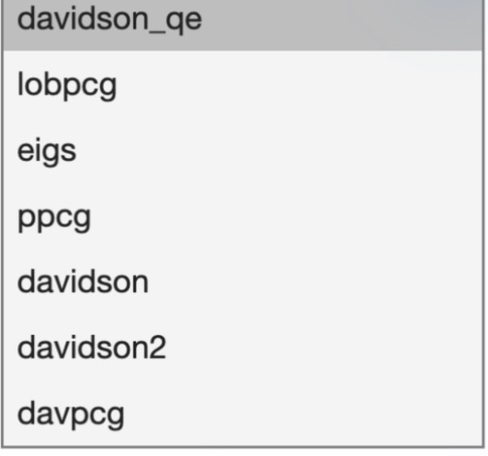
\includegraphics[width=48mm]{publication-assets/crop-1581def0867bec552a40.png}
\caption{SCF節點的演算法列表，本例選擇davidson\_qe。}
\label{fig:h2-scf-methods}
\end{figure}

選中 \ui{Calculate force}。原子力表示在當前電子分佈下，原子沿哪個方向移動會降低能量。本章先不移動原子，計算力是為了在後面的最佳化教程中比較起點和終點。若不需要原子力，普通單點能計算可以不勾選這一項。

高階選項中的 \ui{ExxMethod} 保持 \ui{default}。它主要服務於雜化泛函計算，不需要在本例的 PBE 計算中額外調整。

完成填寫後，按表\ref{tab:h2-scf-options}逐項核對。較長的方法名可以在最大化的配置編輯器中閱讀，核對後再還原佈局。

\begin{table}[!htb]
\centering
\caption{氫分子教程的 SCF 節點引數}
\label{tab:h2-scf-options}
\begin{tabularx}{\linewidth}{lX}
\toprule
選項 & 本例設定\\
\midrule
\ui{DiagMethod} & \ui{davidson\_qe}，每一步求解電子態所用的方法\\
\ui{Max SCF steps} & \texttt{100}，電子密度更新的最大步數\\
\ui{Calculate force} & 選中，在本次單點計算中求原子力\\
\ui{ExxMethod} & \ui{default}，本例保持高階選項的預設設定\\
\bottomrule
\end{tabularx}
\end{table}

\subsection{檢查曲線節點}

能量曲線任務負責把 SCF 的歷史記錄畫成圖，在本例畫布上標為\ui{Plot}。它不再求一次電子結構，也不改變上一步的結果。確認它位於 SCF 之後即可。如果先執行 SCF，隨後才新增曲線節點，可以再次執行這條完整的小工作流，得到與該次計算對應的曲線。

在執行前儲存專案。以後比較不同截斷能、不同結構或不同泛函時，儲存的工作流便是說明計算條件最直接的記錄。

\section{執行計算並觀察進度}

\subsection{選擇正確的工作流}

應用中可以同時開啟多個工作流文件。執行之前，先點選本例工作流的文件標籤，讓它成為當前工作流，再選擇 \ui{執行}。這樣可以避免模型已經切換而執行的仍是另一張工作流的情況。

執行前展開右側面板組，再展開\ui{模擬瀏覽器}的標題欄；如果面板已經關閉，可從\ui{開啟面板}列表中按名稱開啟。配置編輯器仍佔滿工作區時，先用標題欄選單\ui{還原}，便可同時觀察畫布和輸出。執行後，這裡開始顯示計算訊息。SCF 日誌通常按迭代步依次列出誤差、總能量和耗時。某一步的誤差下降較慢，並不意味著操作有誤；判斷整個計算時，應檢視完整的迭代過程和最終的收斂狀態。

\begin{steps}
\item 使氫分子的 SCF 工作流處於當前文件。
\item 選擇 \ui{主頁 → 執行}，或使用模擬瀏覽器中的 \ui{執行} 按鈕。
\item 在模擬瀏覽器中找到氫分子計算開始的訊息。
\item 等待出現收斂訊息，隨後檢視自動開啟的曲線。
\item 返回工作流畫布，確認需要執行的節點已經完成。
\end{steps}

本地\ui{停止}按鈕只恢復執行按鈕狀態，不會中斷正在進行的數值求解；線上版同步計算也不提供停止操作。本例應等待計算結束後再繼續。執行期間可檢視日誌判斷進度，關閉瀏覽器標籤不會儲存專案或結束伺服器計算。

\subsection{測量一次執行的用時}

\ui{執行}右側的下拉選單提供\ui{執行並計時}。先啟用本章SCF流程，再選擇該項；本地流程完成後，視窗底部顯示本次用時。計時包含這次流程的執行和相關準備，不是每個節點的獨立效能分析。

比較用時之前，保持模型、引數和執行環境一致，並說明是否首次執行。首次開啟數值功能或生成圖形可能增加準備時間。使用遠端配置提交作業時，本地提交耗時不等於遠端計算耗時，應閱讀遠端作業的記錄。儲存本章專案時，可以將計時另記在實驗筆記中，科學結果仍以能量、誤差與收斂狀態判斷。


\subsection{理解日誌中的三個數字}

第一次閱讀日誌時，先關注迭代編號、相對密度誤差和總能量。迭代編號表明求解器進行了多少次更新；密度誤差反映前後兩次電子密度的差別；總能量則是當前密度下對體系能量的估計。

電子密度逐漸自洽時，總能量往往趨於穩定，但能量序列不一定嚴格單調。求解器會混合歷史密度以加快收斂，因此某一步能量稍有回升仍可能是正常的數值過程。判斷是否完成，應讀最終的收斂資訊，而不是隻看最後兩行能量是否相同。

\begin{figure}[!htb]
\centering
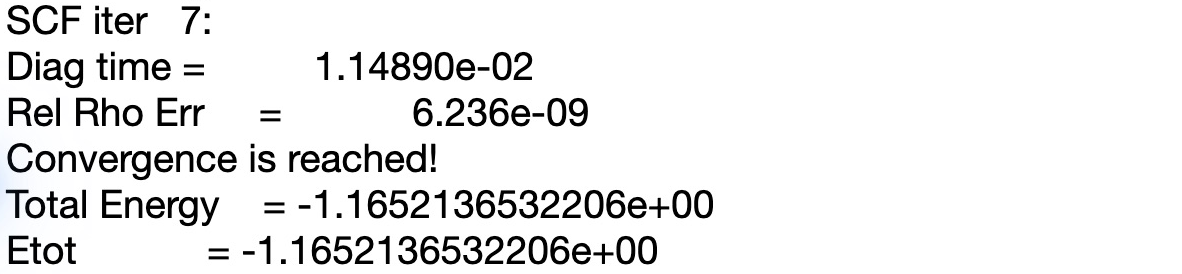
\includegraphics[width=119.9mm]{publication-assets/crop-2984400ea30d3f4eb1f5.png}
\caption{氫分子SCF計算的日誌區域性。第7步出現\ui{Convergence is reached!}，總能量為$-1.1652136532206$ Ha，相對密度誤差約為$6.24\times10^{-9}$。}
\label{fig:h2-scf-runtime-log}
\end{figure}

\section{閱讀第一幅計算結果}

\subsection{讀懂收斂曲線}

收斂圖把同一次 SCF 的兩類記錄畫在一起。橫軸是迭代次數，左縱軸為總能量，單位 Ha；右縱軸為誤差。誤差軸使用對數刻度，因此相同的縱向距離可以對應誤差相差一個或多個數量級。

觀察圖形時，可以先沿著能量曲線從左往右閱讀，再看誤差是否整體降低。對於這個很小的氫分子，能量在開始幾步便接近穩定，誤差仍需進一步下降。這說明“圖上看起來已經平了”和“求解器已經達到收斂條件”是兩個不同的判斷。

\begin{figure}[!htb]
\centering
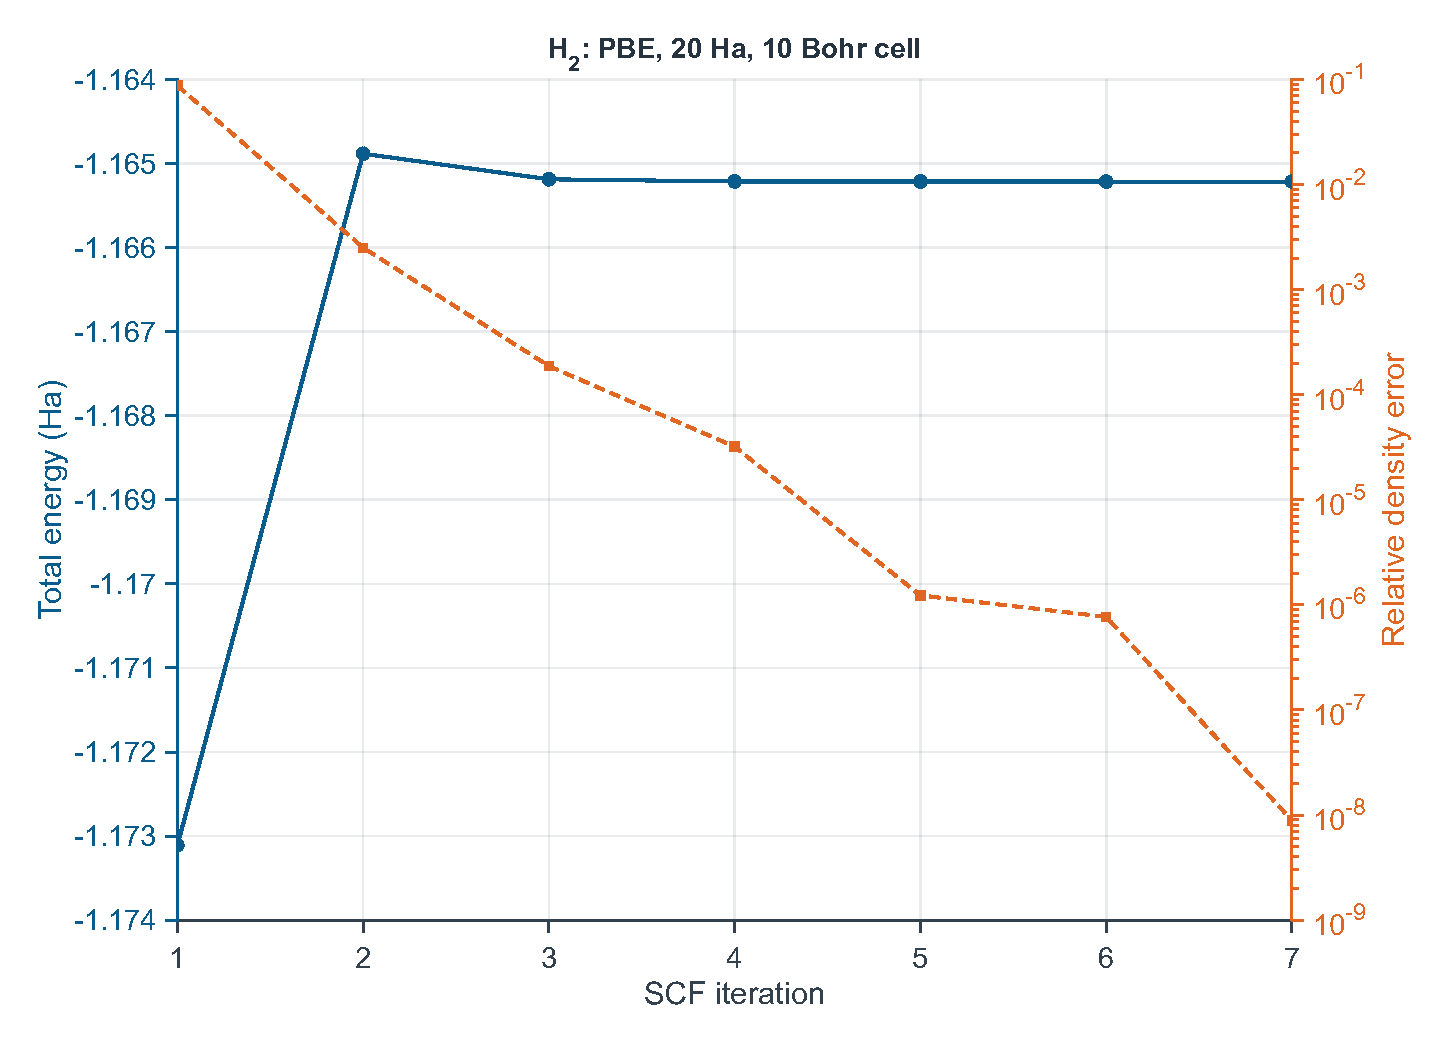
\includegraphics[width=\linewidth]{publication-assets/vector-2e572f3c8654292658e8.pdf}
\caption{氫分子自洽計算的總能量與相對密度誤差。藍線讀左軸，橙色虛線讀右側對數軸；圖中資料來自隨書參考執行。}
\label{fig:h2-scf-results}
\end{figure}

\subsection{與本書的參考執行比較}

隨書指令碼給出的參考結果在 $7$ 步達到收斂，總能量約為 $-1.1652136531$ Ha，最後的相對密度誤差約為 $8.85\times10^{-9}$。可以用這些數值對照自己的計算結果。

圖\ref{fig:h2-scf-runtime-log}所示計算同樣在7步後收斂，總能量約為$-1.1652136532$ Ha，相對密度誤差約為$6.24\times10^{-9}$。兩組計算均滿足本例的收斂條件。圖\ref{fig:h2-scf-results}展示隨書指令碼儲存的能量與誤差歷史。

在圖形介面中執行時，初始電子態、軟體版本和數值環境可能使迭代次數或最後幾位數字略有不同。比較時先確認結構、盒尺寸、泛函、贗勢和截斷能一致，再檢查最終是否收斂。執行時間還受裝置和會話負載影響，判斷結果應以收斂狀態和數值為依據。

\begin{notebox}{總能量的含義}
本例的總能量屬於這個盒中、這個幾何構型、這套泛函和贗勢條件下的氫分子。它不直接等於實驗中的分子結合能。若要計算解離能，還需要以一致的方法計算相應的原子參考態，並處理自旋等條件。
\end{notebox}

\subsection{儲存結果和專案}

計算曲線加入專案的結果分類後，可以從專案瀏覽器再次開啟。圖形是計算記錄的一種呈現，工作流儲存的是產生它的步驟，兩者都有保留的價值。建議在執行後再次儲存專案，而不只是在執行前儲存一次。

為圖形使用容易理解的名稱，例如“氫分子：PBE，20 Ha，初始結構”。如果後面還要計算最佳化後的結構，清楚的名稱可以避免把兩個構型的結果混在一起。名稱中可以放主要條件，完整引數則留在工作流中，不必把所有內容塞進一個很長的檔名。

\section{完成本章練習}

重新開啟儲存的專案，確認結構、工作流中的結構選擇和結果圖都能恢復。

作為延伸練習，再次匯入\file{h2.cif}，命名為\file{H2-longer}。按第~\ref{ch:modeling}~章的幾何編輯方法，將鍵長設為$0.85\,\text{\AA}$；隨後回到\ui{Build Molecule}，在\ui{Choose imported structures}中改選這一結構，保持截斷能、泛函和模擬盒不變，再執行單點計算。分別儲存兩次結果，比較總能量和沿鍵方向的力。第~\ref{ch:workflows}~章繼續介紹幾何最佳化，第~\ref{ch:results}~章介紹結果解讀。

\section{用指令碼復現本例}

本節面向使用完整 MATLAB\regmark{} 的讀者。獨立應用和線上版可以繼續使用前面的圖形操作，無需執行配套指令碼。圖形介面便於學習和檢查結構，指令碼便於重複執行相同引數。配套 \file{examples/h2_scf_and_relax.m} 給出完整輸入；下面摘錄其中的單點計算部分。此段程式碼用於已經初始化 KSSOLV 數值環境的 MATLAB\regmark{} 會話。

\Needspace{11\baselineskip}
\begin{lstlisting}[language=Matlab]
pseudopotential.PpType('default');
molecule = example.structure.H2();
molecule.ecut = 20;
molecule.funct = 'PBE';
scfOptions = options.SCF('force', true);
scfOptions.enableGPU = false;
scfOptions.enableParallelPool = false;
[molecule, H, X, info] = scf(molecule, scfOptions);
\end{lstlisting}

返回值中，\texttt{info.Etot}是總能量，\texttt{info.Etotvec}和\texttt{info.SCFerrvec}記錄能量與誤差歷史，\texttt{info.converge}給出收斂狀態，可用於整理表格或繪圖。配套指令碼還會繼續最佳化原子位置並儲存資料；只重複本章時，執行上述單點部分即可。圖形介面與指令碼採用同一數值模型，操作時沿用本例明確給出的引數。

